\documentclass{article}
\usepackage{graphicx}
\usepackage{physics}
\usepackage{amsmath}
\graphicspath{{./Figures/}}

\begin{document}

\title{Two Charged Black Hole problem}
\author{Joseph Lannan}

\maketitle

\begin{abstract}
Imagine two black holes both with the same charge sitting in equilibrium between the gravitational field and the electric. Now if we were to move into a moving reference frame, some of that electric field would create a magnetic field and we would see a outward force acting on two charges due to this magnetic field. The two particles should however still remain in equilibrium so that there's still no net force acting on either particle. So using a classical analogy, there must be some magnetic component of the gravitational field that is created in a moving reference frame. 
\end{abstract}

\section{Transforms on the Electric field}
So to begin understanding this system, lets start with looking at just the transforms acting on the electric field. First we need to define the Electromagnetic tensor:
\begin{equation}
	F_{\mu \nu} = \partial_\mu A_\nu - \partial_\nu A_\mu
\end{equation}
Where A is the four-potential such that
\begin{equation}
	A^\alpha = (\phi/c,A)
\end{equation}
In relation to the usual E and B fields, we can write this as
\begin{equation}
	E = - \nabla \phi - \frac{\partial \vec{A}}{\partial t}
	B = \nabla x \vec{A}
\end{equation}

\begin{equation}
	F = \begin{bmatrix}
		0 & -E_x/c & -E_y/c & -E_z/c \\
		E_x/c & 0 & -B_z & B_z \\
		E_y/c & B_z & 0 & -B_x \\
		E_z/c & -B_y & B_x & 0
	\end{bmatrix}
\end{equation}
Note that this matrix is anti-symmetric and that there may be an overall minus to this depending on how the Minkowski metric is defined.
Now using this we can operate on it using Lorentz transforms in the usual manor:
\begin{equation}
	F'^{\mu \nu}= \Lambda^\mu_\nu F^{\mu \nu} \Lambda^\nu_\mu
\end{equation}
Luckly we don't have to care to much about the variance here since both the Lambdas are symmetric. Doing this operation in Matlab we can do this for a lot of different points throughout a space and make some interesting graphs to visualize the effect.
in \ref{fig:untransformed} we can see the field that is generated by a point charge before we apply our transformation. There is no magnetic field counterpart to this charge since we are in the rest frame. The velocity these were transformed to was $.5c$ to make the effects much more obvious.

\begin{figure}[h!]
  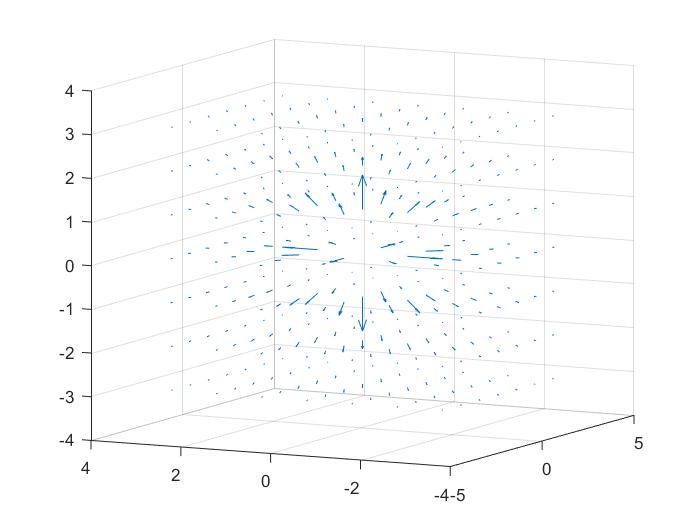
\includegraphics[width=100mm,scale=.5]{untransformed.jpg}
  \caption{Electric field of a Point Charge in the Rest Frame}
  \label{fig:untransformed}
\end{figure}

Now going to a moving reference frame, we can see the effects on the fields in \ref{fig:etransformed} and \ref{fig:btransformed}

\begin{figure}[h!]
  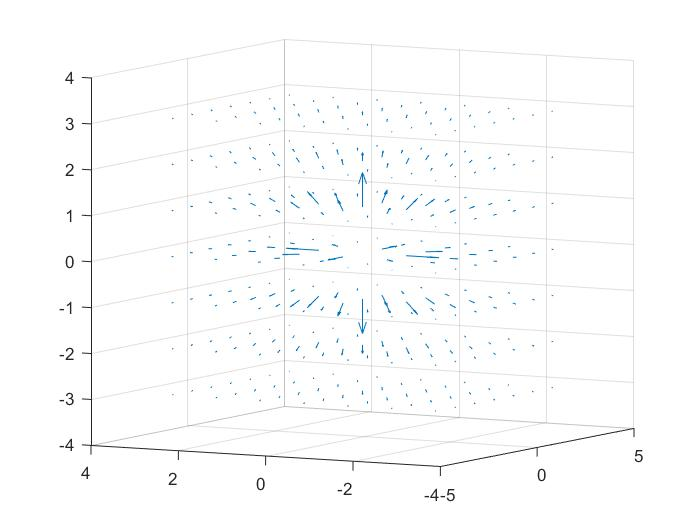
\includegraphics[width=100mm,scale=.5]{electrictransformed.jpg}
  \caption{Electric field of a Point Charge in the Moving Frame}
  \label{fig:etransformed}
\end{figure}

\begin{figure}[h!]
  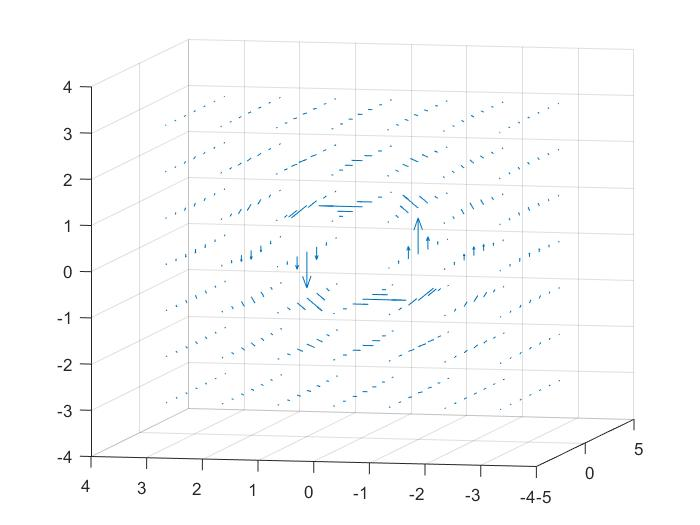
\includegraphics[width=100mm,scale=.5]{magnetictransformed.jpg}
  \caption{Magnetic field of a Point Charge in the Moving Frame}
  \label{fig:btransformed}
\end{figure}

Now we more particularly care about the case of two dipole charges being transformed in the context of our problem. Here  are the same results but for a dipole charge.

\begin{figure}[h!]
  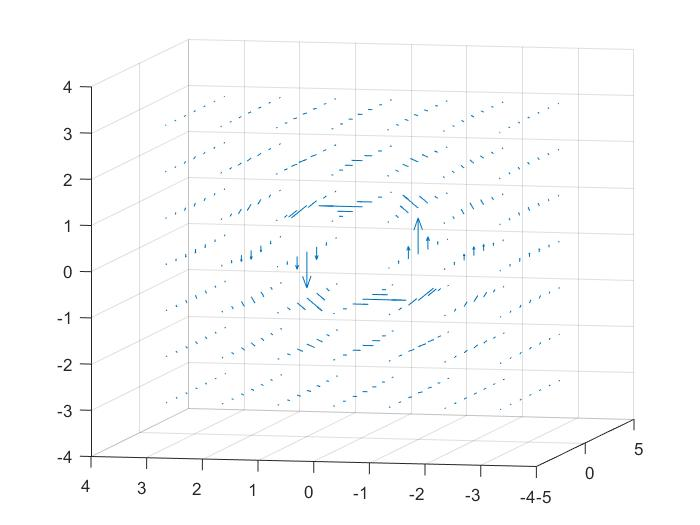
\includegraphics[width=100mm,scale=.5]{magnetictransformed.jpg}
  \caption{Magnetic field of a Point Charge in the Moving Frame}
  \label{fig:btransformed}
\end{figure}

\end{document}